\subsection{Overview}
% High-level components and their interaction
% TODO: @Hrvoje
\subsection{Component view}
In the following section, components used to implement different functionalities of the system is described, aided with component diagrams demonstrating their separation and interactions within each other and with other external interfaces.
\begin{figure}[H]
    \centering
    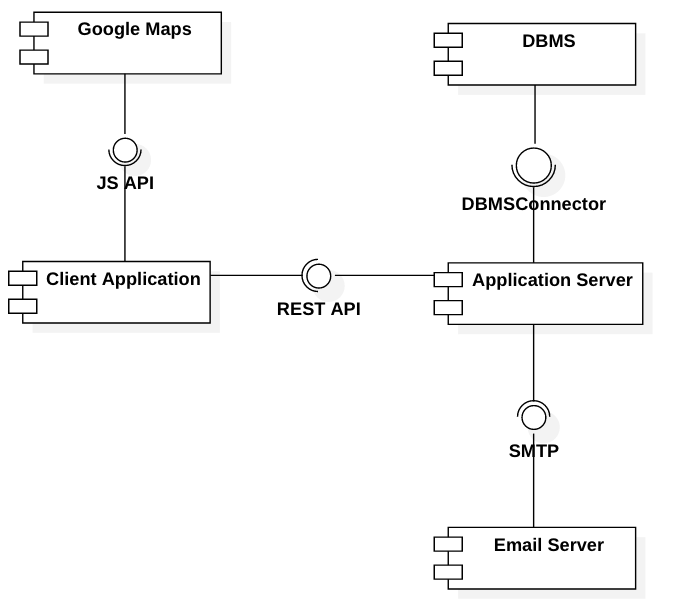
\includegraphics[height=0.4\textwidth]{Images/ComponentDiagrams/Overall.png}
    \caption{Component Diagram for the overall system}
    \label{fig:CDOverall}
\end{figure}
\nameref{fig:CDOverall} provides an overall view to the components present in the system and the connections between these components to correctly realize the decisions provided in this document.
The external integrations of the system, with the general communication interfaces they communicate with other components are provided, however the details for the Application Server will be presented following, only, considering that the main application logic is executed through the components residing in it.
The client is a thin-client built to interact with and display information directly sent through the endpoints.
Therefore, it is provided as one component that is unnecessary to split into sub-components.
\begin{figure}[H]
    \centering
    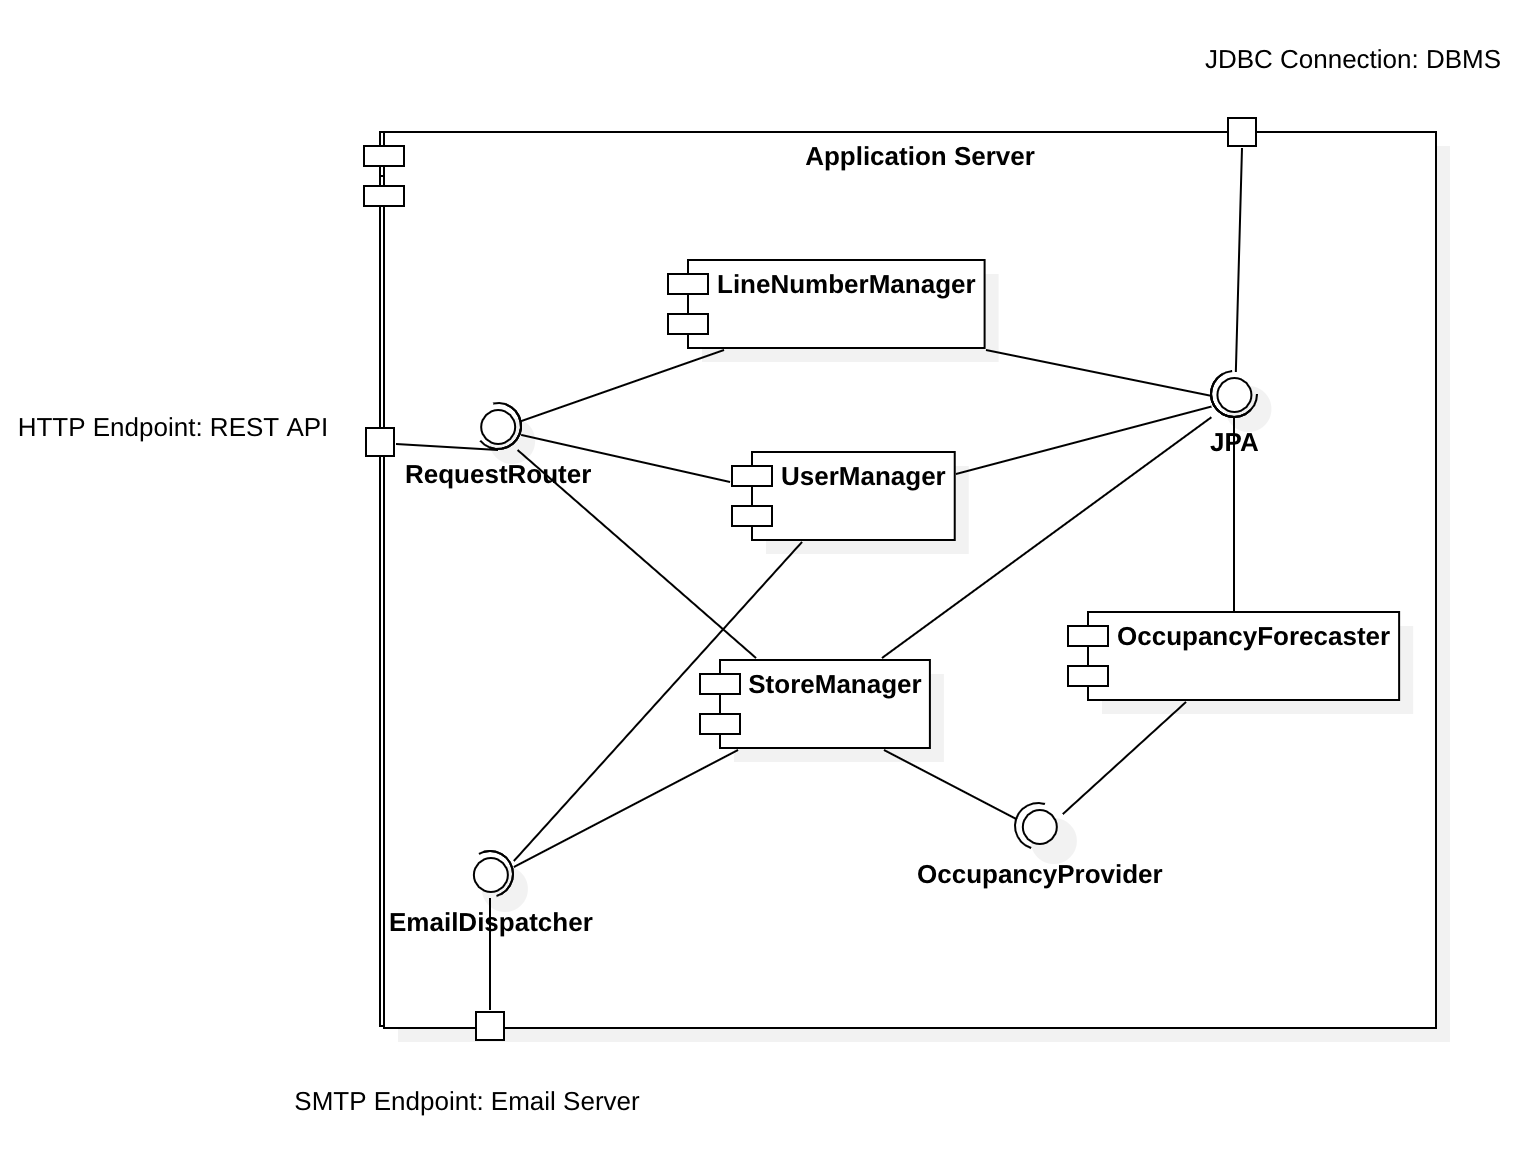
\includegraphics[height=0.4\textwidth]{Images/ComponentDiagrams/ApplicationServer.png}
    \caption{Component Diagram for the Application Server}
    \label{fig:CDApplicationServer}
\end{figure}
\nameref{fig:CDApplicationServer} provides an overall view for the components inside the Application Server.
The components separate the functionality into three domains, namely Line Numbers, Users and Stores.
All other entities that exist in the system are included into one of these domains based on their relevance.
All the user facing functionalities of the system are exposed through the REST endpoint, which uses a router interface to route each request to the domain component it belongs to.
All domain components use JPA to persist their domain data structures, and components that require to send e-mails use the SMTP endpoint to do so.
The OccupancyForecaster is a component that features only one function: periodically reading the database for entry and exit records of customers and updating the store accordingly.
Therefore, it is not split further into components.
\begin{figure}[H]
    \centering
    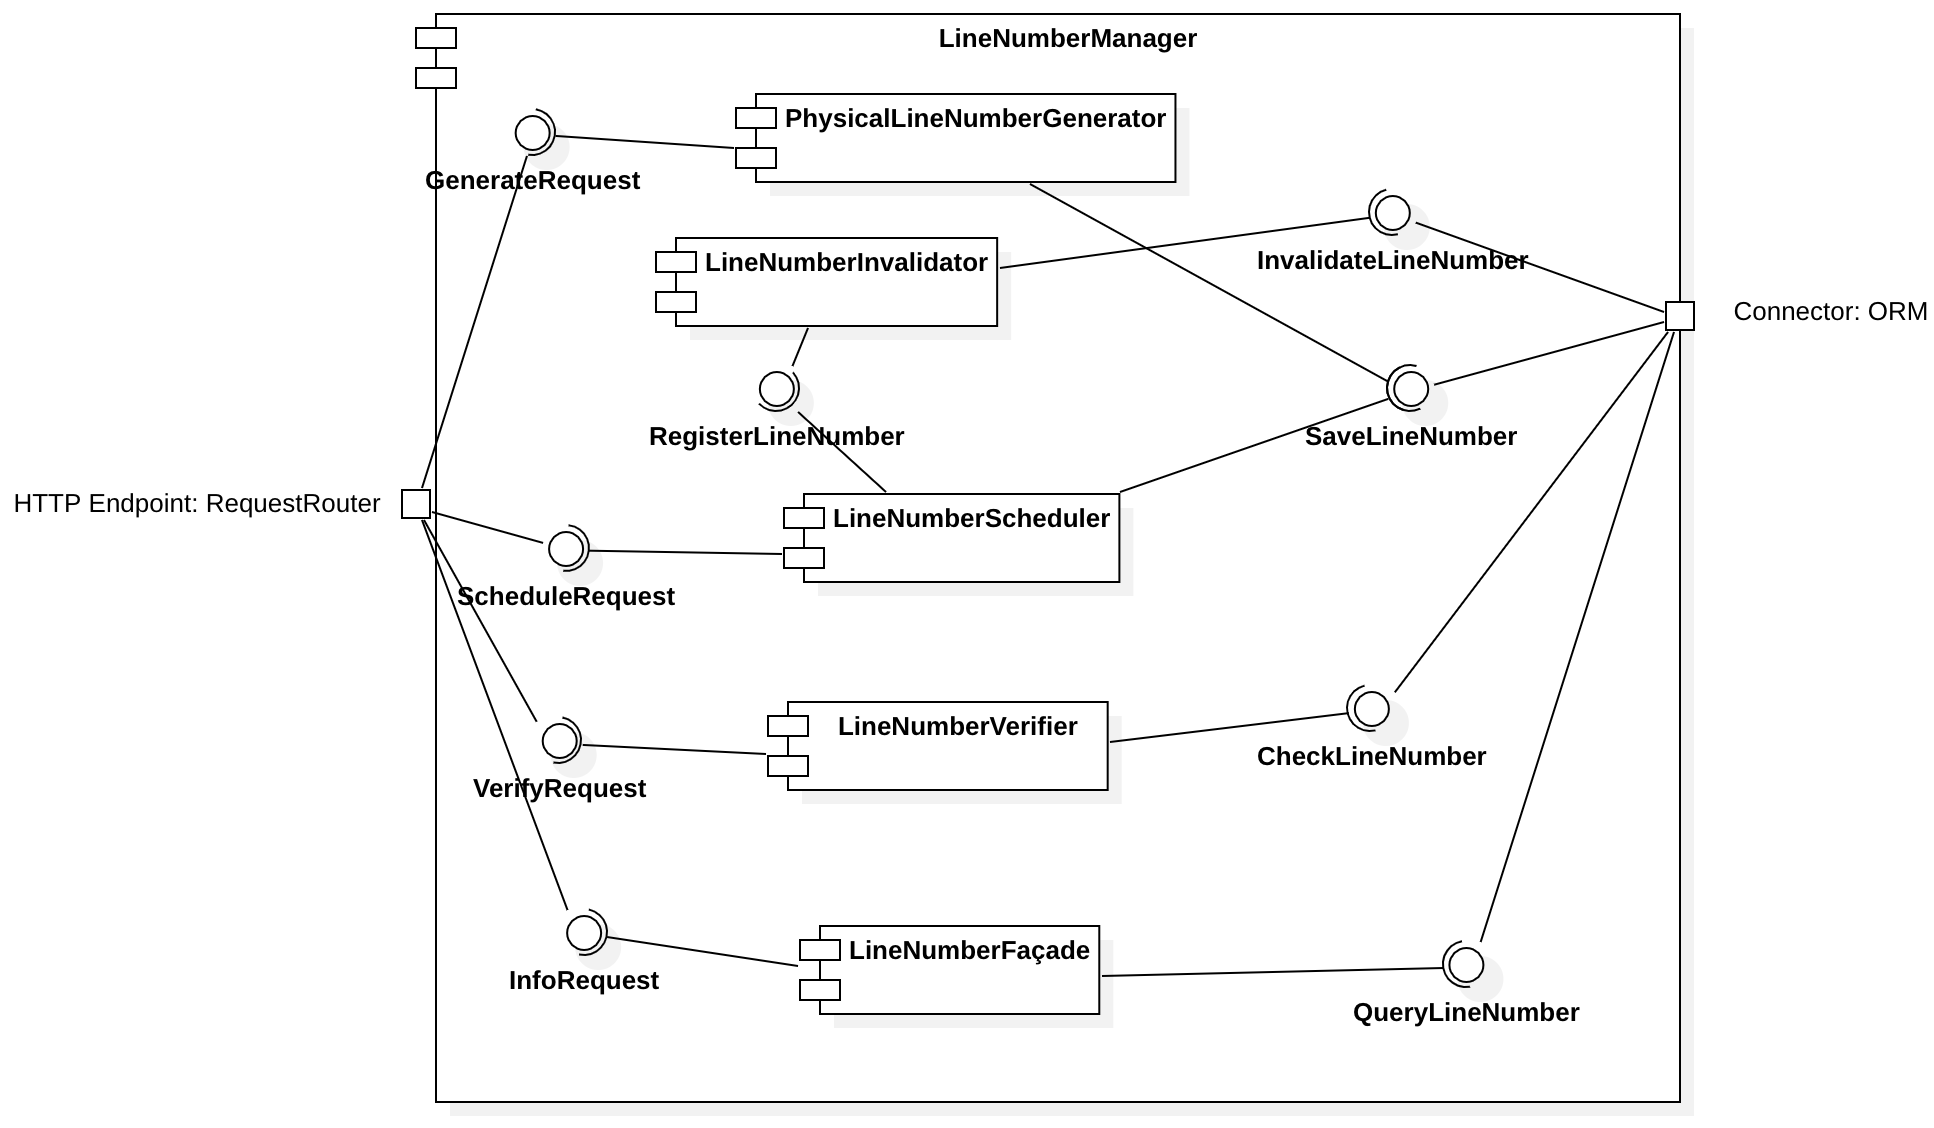
\includegraphics[height=0.4\textwidth]{Images/ComponentDiagrams/LineNumberManager.png}
    \caption{Component Diagram for the LineNumberManager}
    \label{fig:CDLineNumberManager}
\end{figure}
\nameref{fig:CDLineNumberManager} provides a detailed view over the domain component for line numbers.
It allows the management of any sort of query related to line numbers by clerks and customers.
This component is further divided into following sub-components to increase the granularity of actions performed on line numbers:
\begin{itemize}
    \item \textbf{PhysicalLineNumberGenerator}: This component exists to provide an interface for clerks to generate line numbers, it's interface handles the incoming request by generating and persisting a new ticket for the to-be-printed line number.
    \item \textbf{LineNumberScheduler}: This component exists to allow the users of the system to book a line number from their home.
    It realizes its functionality through connecting to the same interface of the persistence provider, however it is capable of handling more complex requests, including custom product or category selection and time slot allocation.
    Furthermore, it registers the ticket to the LineNumberInvalidator to be invalidated after the set timeout minutes have passed from the time slot.
    \item \textbf{LineNumberInvalidator}: This component acts as a helper component to LineNumberScheduler.
    It schedules the invalidation of the scheduled tickets, so that the invalidation can occur asynchronously.
    This component is created to separate this responsibility from an active user facing component, all which have the main responsibility to provide a synchronous response to all the users' needs.
    \item \textbf{LineNumberVerifier}: This component is used to handle the transactions regarding customer QR code verification conducted by the Clerk.
    It is used to register the entrance and exit of customers with their QR codes.
    \item \textbf{LineNumberFa\c{c}ade}: This component is used by the customers that want to query detailed information regarding the line numbers that they have.
    The requests handled by this endpoint is directly mapped to the client application's needs.

\end{itemize}
\begin{figure}[H]
    \centering
    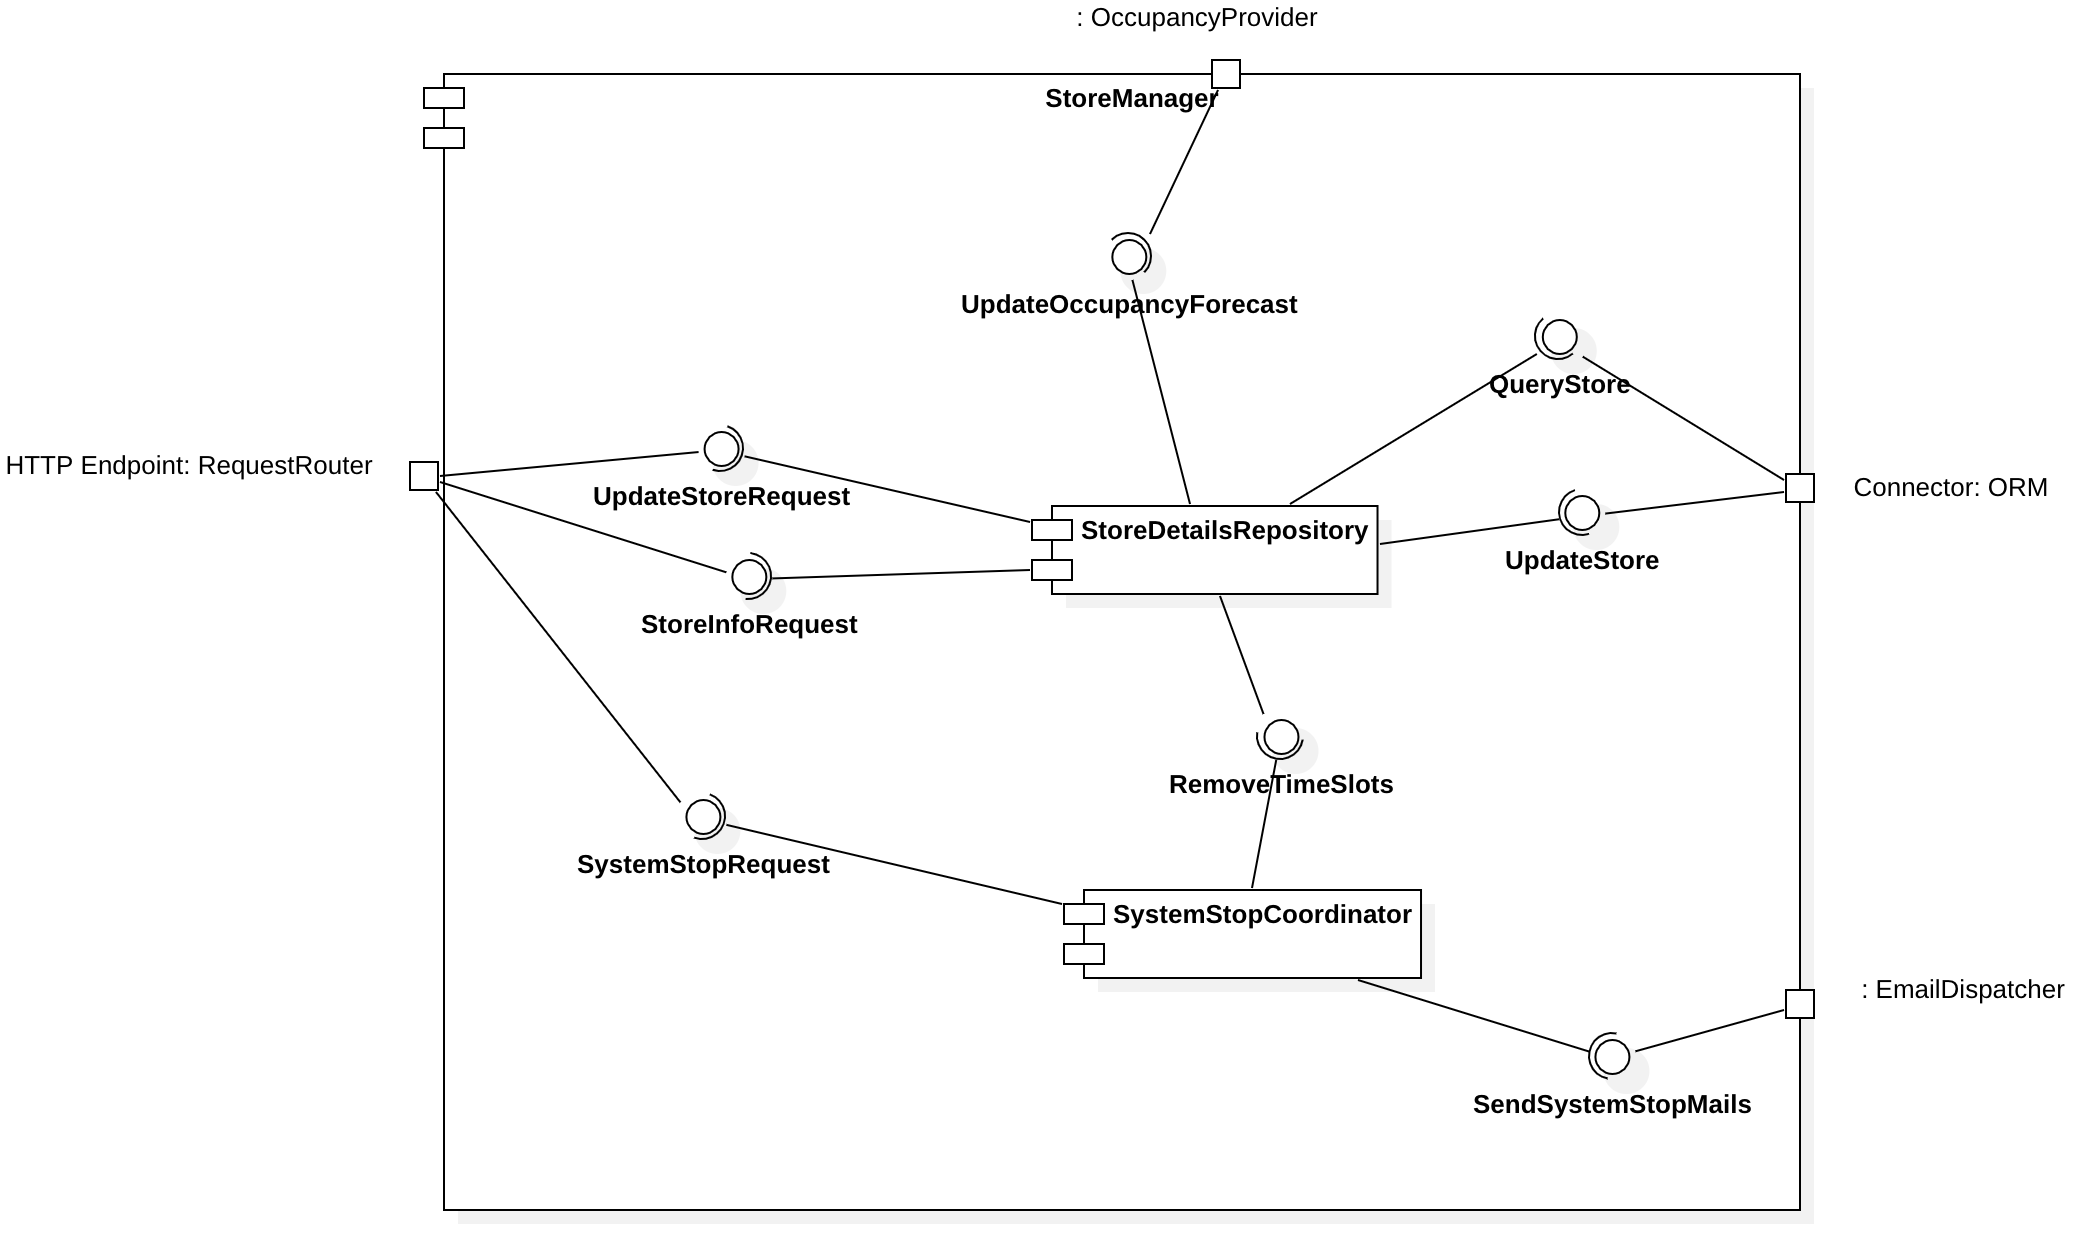
\includegraphics[height=0.4\textwidth]{Images/ComponentDiagrams/StoreManager.png}
    \caption{Component Diagram for the StoreManager}
    \label{fig:CDStoreManager}
\end{figure}
\nameref{fig:CDStoreManager} provides a detailed view over the domain component for handling requests related to the store.
The wrapping component allows querying all relevant information about the store by all, and furthermore, harbors the logic for the manager users to update different aspects related to the store, such as basic information, time slots, configuration and system stop scheduling.
This component, apart from having mailing, routing and database interfaces, exposes an interface to the OccupancyProvider to retrieve updated information about the occupancy forecast. % TODO move to subcomponent
This component is divided into following components to decrease cohesion between tasks to be performed:
\begin{itemize}
    \item \textbf{StoreDetailsRepository}: This component is responsible for carrying out any direct query to the store data and all of the included classes, which are products, categories and time slots.
    There are two exported interfaces available to be used via HTTP.
    The query interface allows all the system users to view relevant information for the store, while the manager has access to the other interface allowing them to update the information.
    The exposed interface to the OccupancyProvider allows the OccupancyForecaster to store updated information regarding the future predictions for the store.
    \item \textbf{SystemStopCoordinator}: This component is responsible for carrying out all the actions that are necessary to perform or schedule a system stop, that are removing the specific time slot and sending e-mails to customers who has already booked those time slots.
\end{itemize}

\begin{figure}[H]
    \centering
    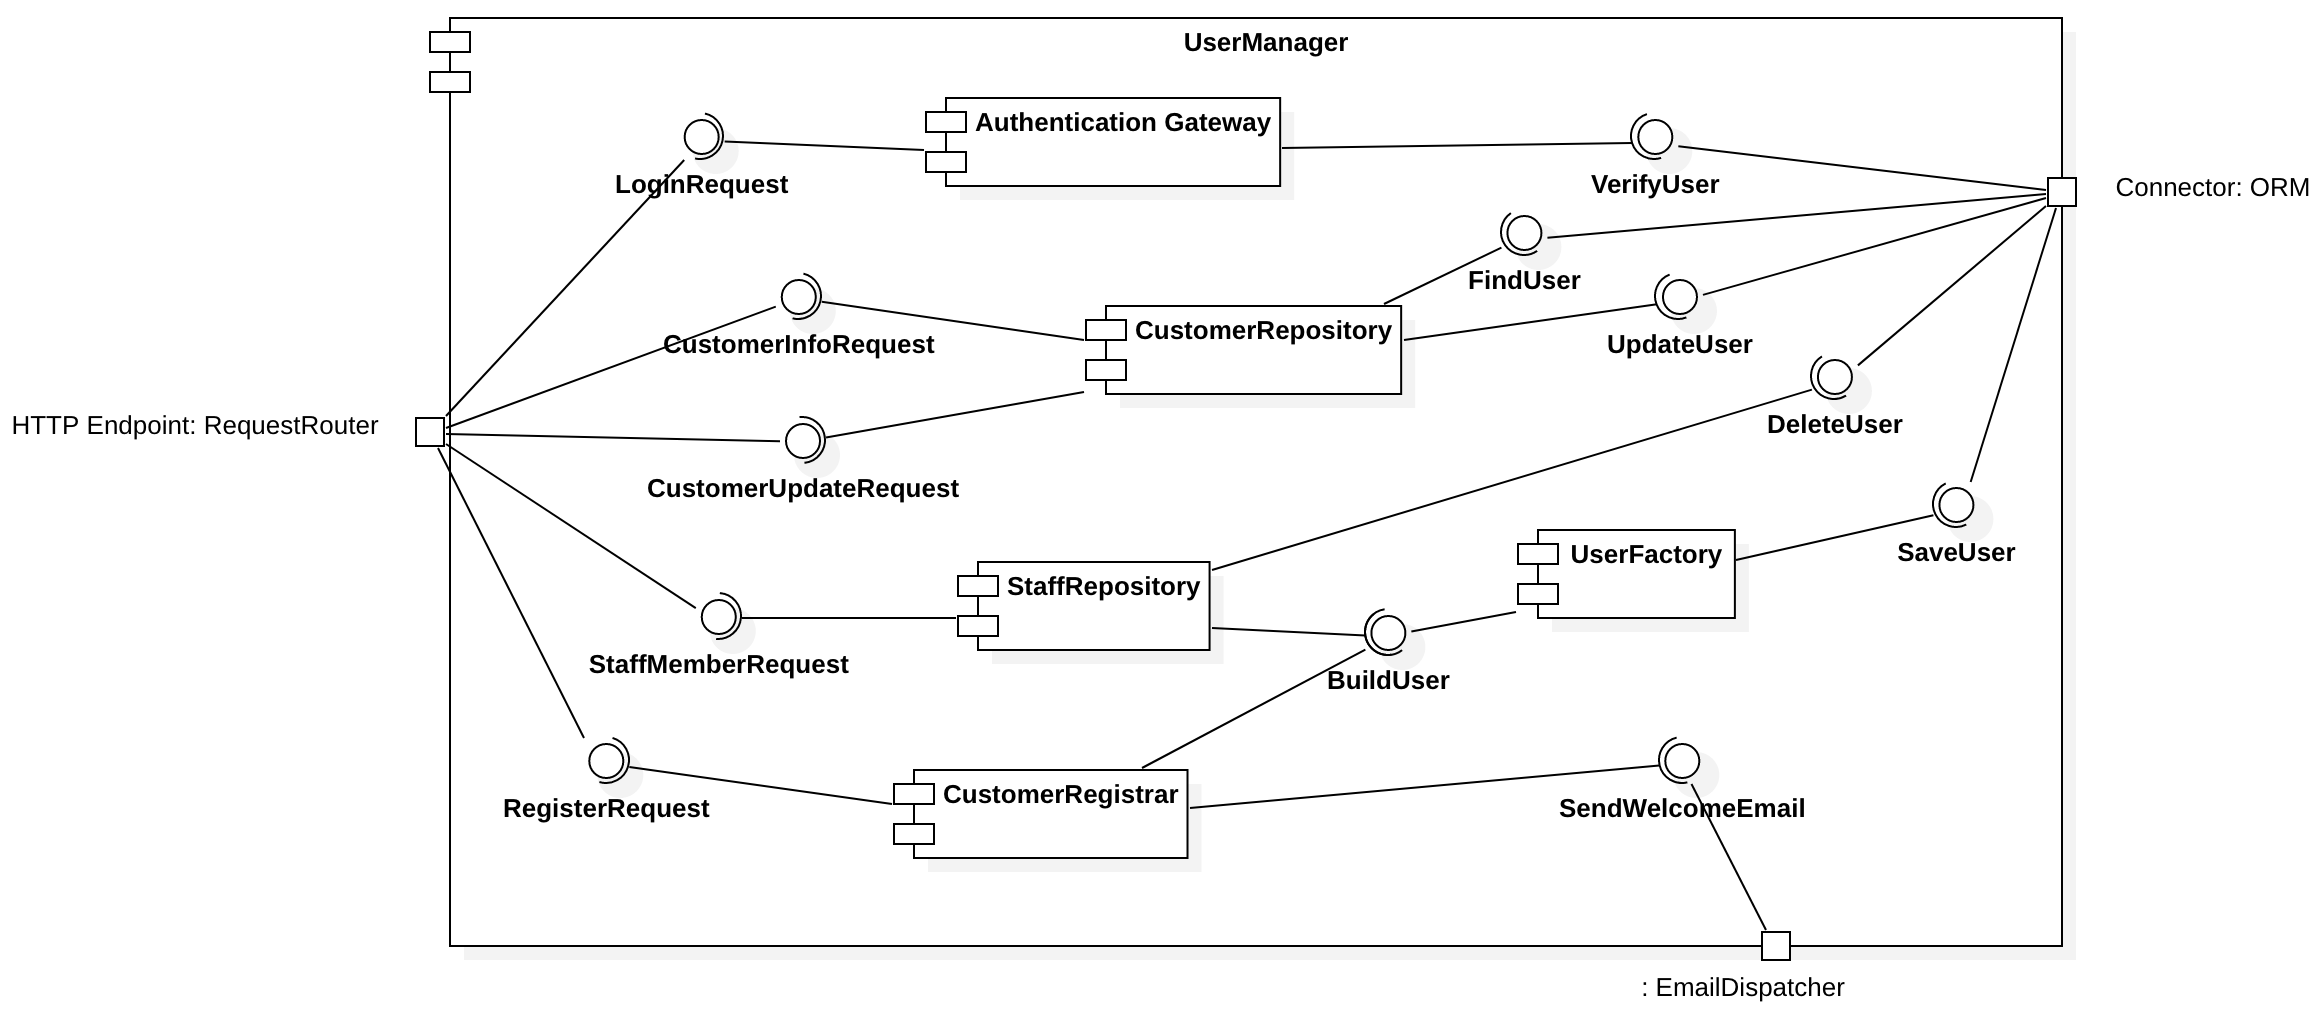
\includegraphics[height=0.4\textwidth]{Images/ComponentDiagrams/UserManager.png}
    \caption{Component Diagram for the UserManager}
    \label{fig:CDUserManager}
\end{figure}
\nameref{fig:CDUserManager} provides a detailed view of the sub-components related to requests that can be performed on users.
This component not only acts as a user registry, but also provides the authentication interfaces required, since its logic encompasses handling user data and authentication is done via user's email address, which relates these functions.
To seperate responsibility on different actions to be performed on the system, this component is divided into specific sub-components, that are:
\begin{itemize}
    \item \textbf{AuthenticationGateway}: This component acts as a medium to authenticate the user and generate the necessary authorization tokens for future use.
    \item \textbf{StaffRepository}: This component handles all the requests related to adding and removing staff members to stores.
    Since, in our design, different flavors of users are implemented using the same basis, the creation and removal of manager and clerks are similar from the architectural point of view.
    Furthermore, since the implementation of user creation is similar to that of the customers, a common factory component is provided to prevent duplication.
    \item \textbf{CustomerRegistrar}: This component handles the requests specific to registering new customers into the system.
    The component is responsible for calling the shared UserFactory to create a customer user and send the customer a welcome email.
    \item \textbf{UserFactory}: This component acts as a common interface and as a factory to create users.
    It is used by the components mentioned above to introduce new users to the system.
\end{itemize}
% Component diagram combining all components and each component having it's subcomponents in a different diagram with explanations
\subsection{Deployment view}
% Deployment diagram with explaining each tier
The following diagram illustrates the physical architecture and the
deployment of the system.
Each node represents a piece of hardware which harbours one or more software units.
Each piece of hardware could be replicated multiple times to improve performances as specified in later in this document.

\begin{figure}[H]
    \centering
    \hspace*{-3.5cm}
    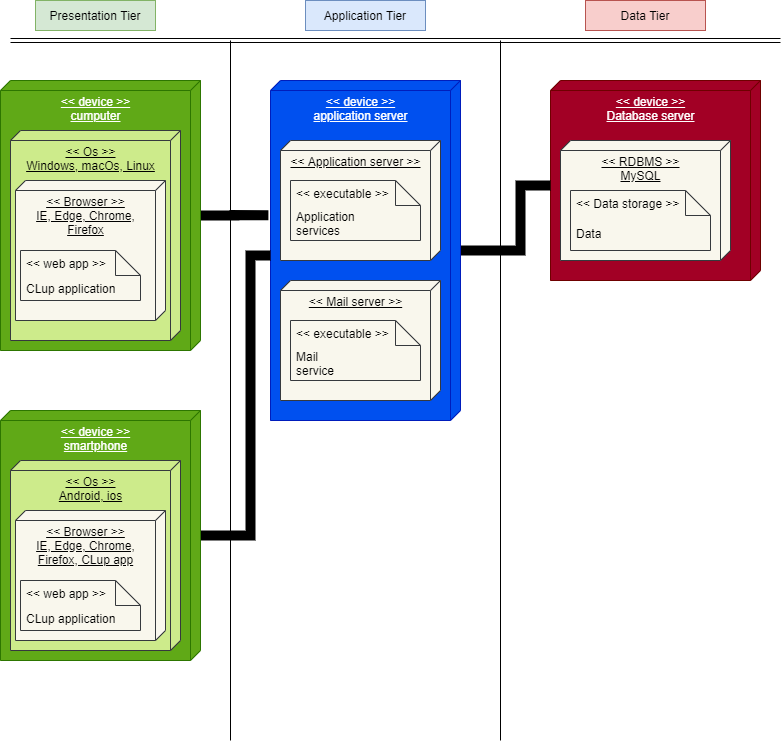
\includegraphics[height=0.7\textwidth]{Images/TierDiagram.png}
    \caption{Deployment view diagram}
\end{figure}

As shown by the diagram, this system is deployed in a three-tier
architecture, where the three tiers consist of: \\
- Presentation tier is the highest-level tier and harbours the presentation logic.
The application is thought to be a web app, so it's accessible from every device with a browser, but it's probable that
a smartphone should be the most used device to access the application so there will be android and ios applications to access
the web app.
The smartphones applications will be more similar to a browser than to a real application, therefore in the diagram is represented asa browser.
In this tier there will not be application logic, so the architecture should be thin-client.\\
- Application tier is the core level from the standpoint of logical management of the application services.
This tier contains all the application logic, from the scheduling of the line numbers to the managment of the store.
This tier is connected to the presentation tier through APIs.
An API is used for each action of the user, and the APIs are divided based on the role of the user.
Each user needs to authenticate using an API and reciving a jwt that needs to be attached to every subsequent request from the same user.
The jwt attached to the request is used to determine wich API are exposed to that user.
This tier contains also a mail Server to notify the users in case their line number is cancelled. \\

- Data tier ( tier 1 in the diagram) is the lowest-level tier as it contains all the information required to fuel the
application services, most prominently the query manager. The
databases are thought to be managed through an RDBMS
(Relational Database Management System), in particular MySQL. Relational databases
have the advantage of having near-maximum information density.
Relational constraints can improve the quality and
integrity of the content of the database.

\subsection{Runtime view}

\subsubsection{Register} % TODO: Text
\subsubsection{Login}% TODO: Text
\subsubsection{Update User Information} % TODO: Graph + Text
% Customer TODO: Roberto
\subsubsection{Book Future Line Number} % TODO: Text
\subsubsection{Retrieve Line Number} % TODO: Text
\subsubsection{View Store} % See location, amount of customers% TODO: Text
% Manager TODO: Ozan
\subsubsection{Add Staff Member}

\begin{figure}[H]
    \centering
    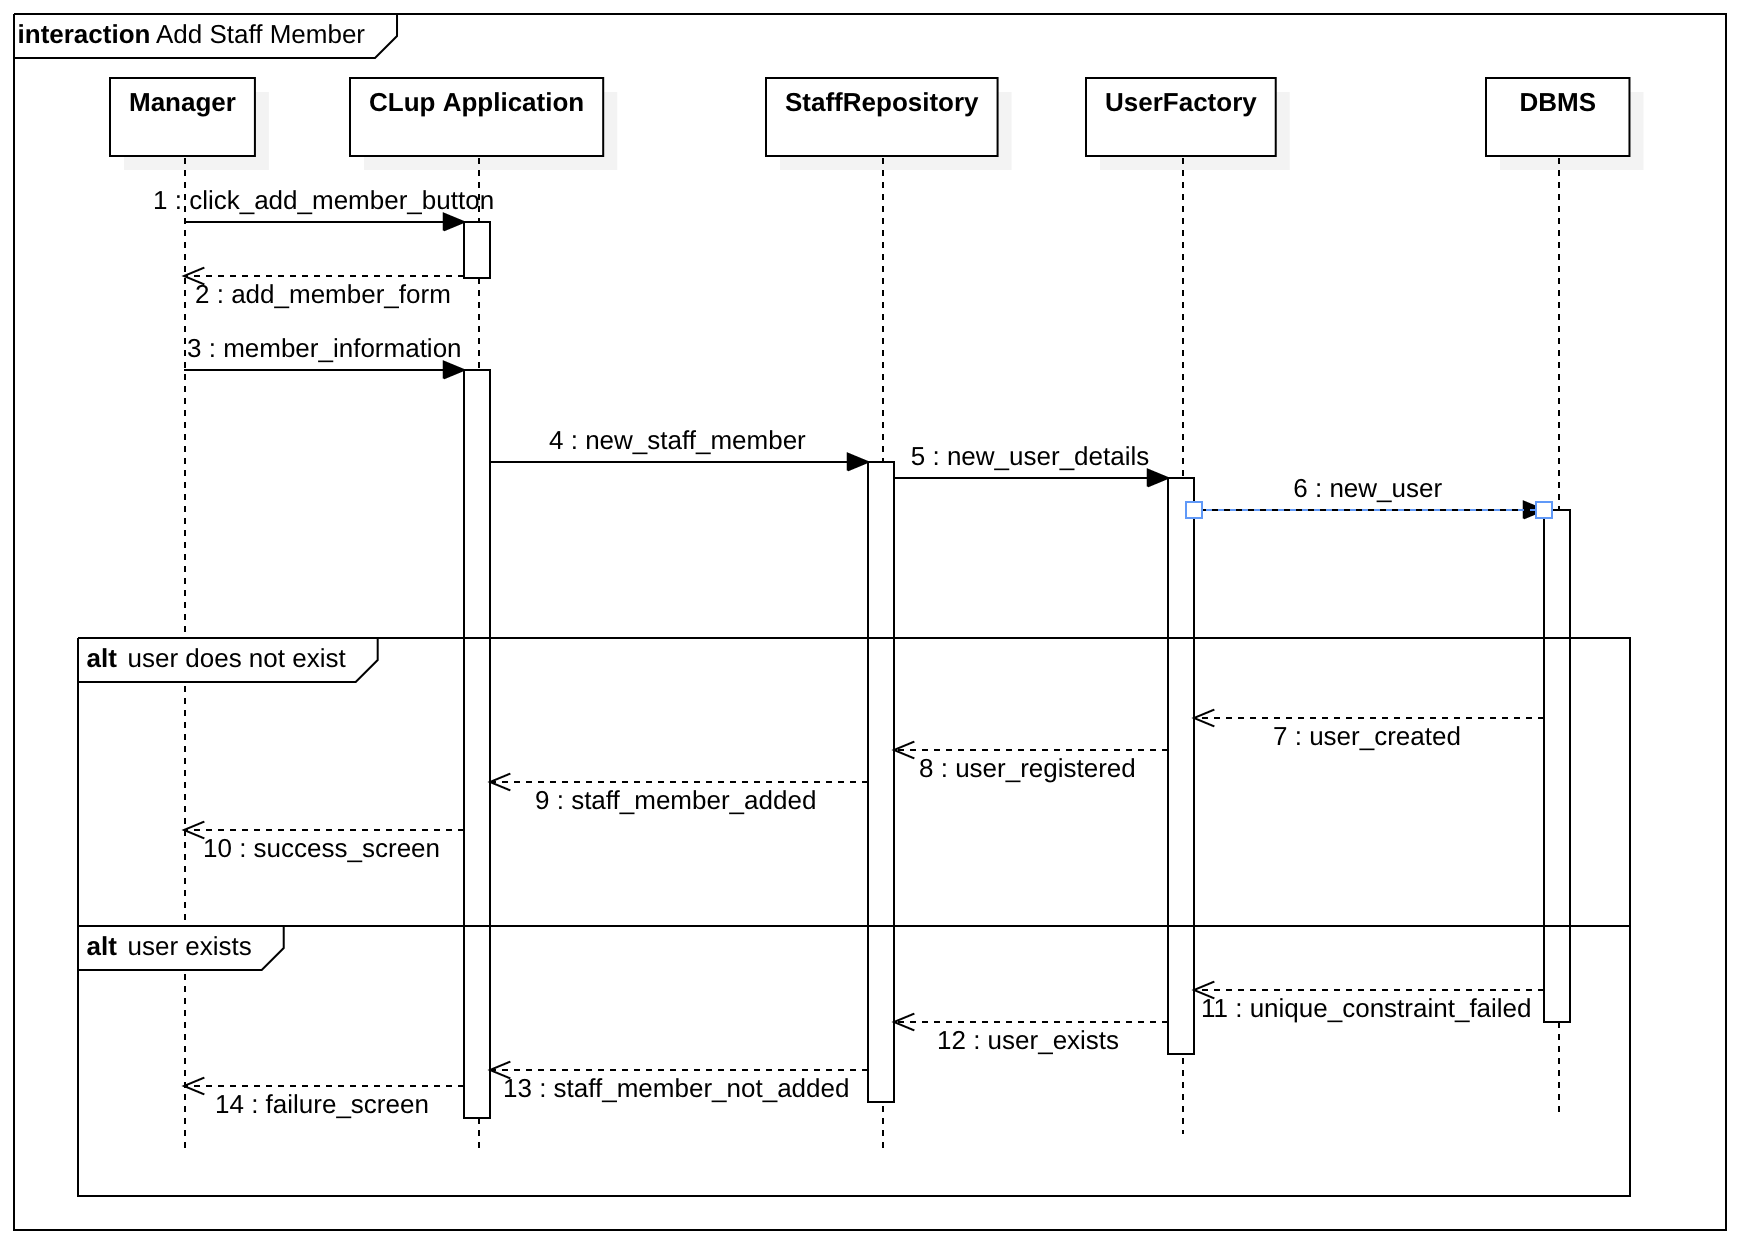
\includegraphics[height=0.4\textwidth]{Images/SequenceDiagrams/AddStaffMember.png}
    \caption{Sequence Diagram for Add Staff Member}
    \label{fig:SDAddStaffMember}
\end{figure}
\nameref{fig:SDAddStaffMember} represents the event flow taking place during the process of adding a new staff member to the store by the manager.
After the manager clicks the "Add Member" button on the application, the application displays a new form featuring the necessary information to create a new staff member user.
When the manager fills in the relevant information and submits the form, the provided information is transferred from the CLup Application to the StaffRepository to be processed.
It shall be noted that the verification of the information (such as valid e-mail address and valid password) is performed within the application, which is not represented in this graph for simplicity.
Upon the retrieval of the information related to the new member to be added, the StaffRepository calls the UserFactory with the information, to create the new user.
The UserFactory then creates the actual user through the DBMS, while applying necessary security measures to the user data, like password hashing.
The DBMS might persist the data given, but it might also fail to do so with a unique constraint failure error, if the provided user credentials is already used by another user.
In case the user didn't exist in the system before the transaction, DBMS emits a message indicating that the user is created, and that message is propagated through the call stack, finally rendering a success screen on the mananger's interface.
However, if the user credentials were already used for another user, the error message emitted by the DBMS gets translated into a simpler form and propagated through the components, with a failure screen shown to the manager.
\subsubsection{Stop for Emergency}
\begin{figure}[H]
    \centering
    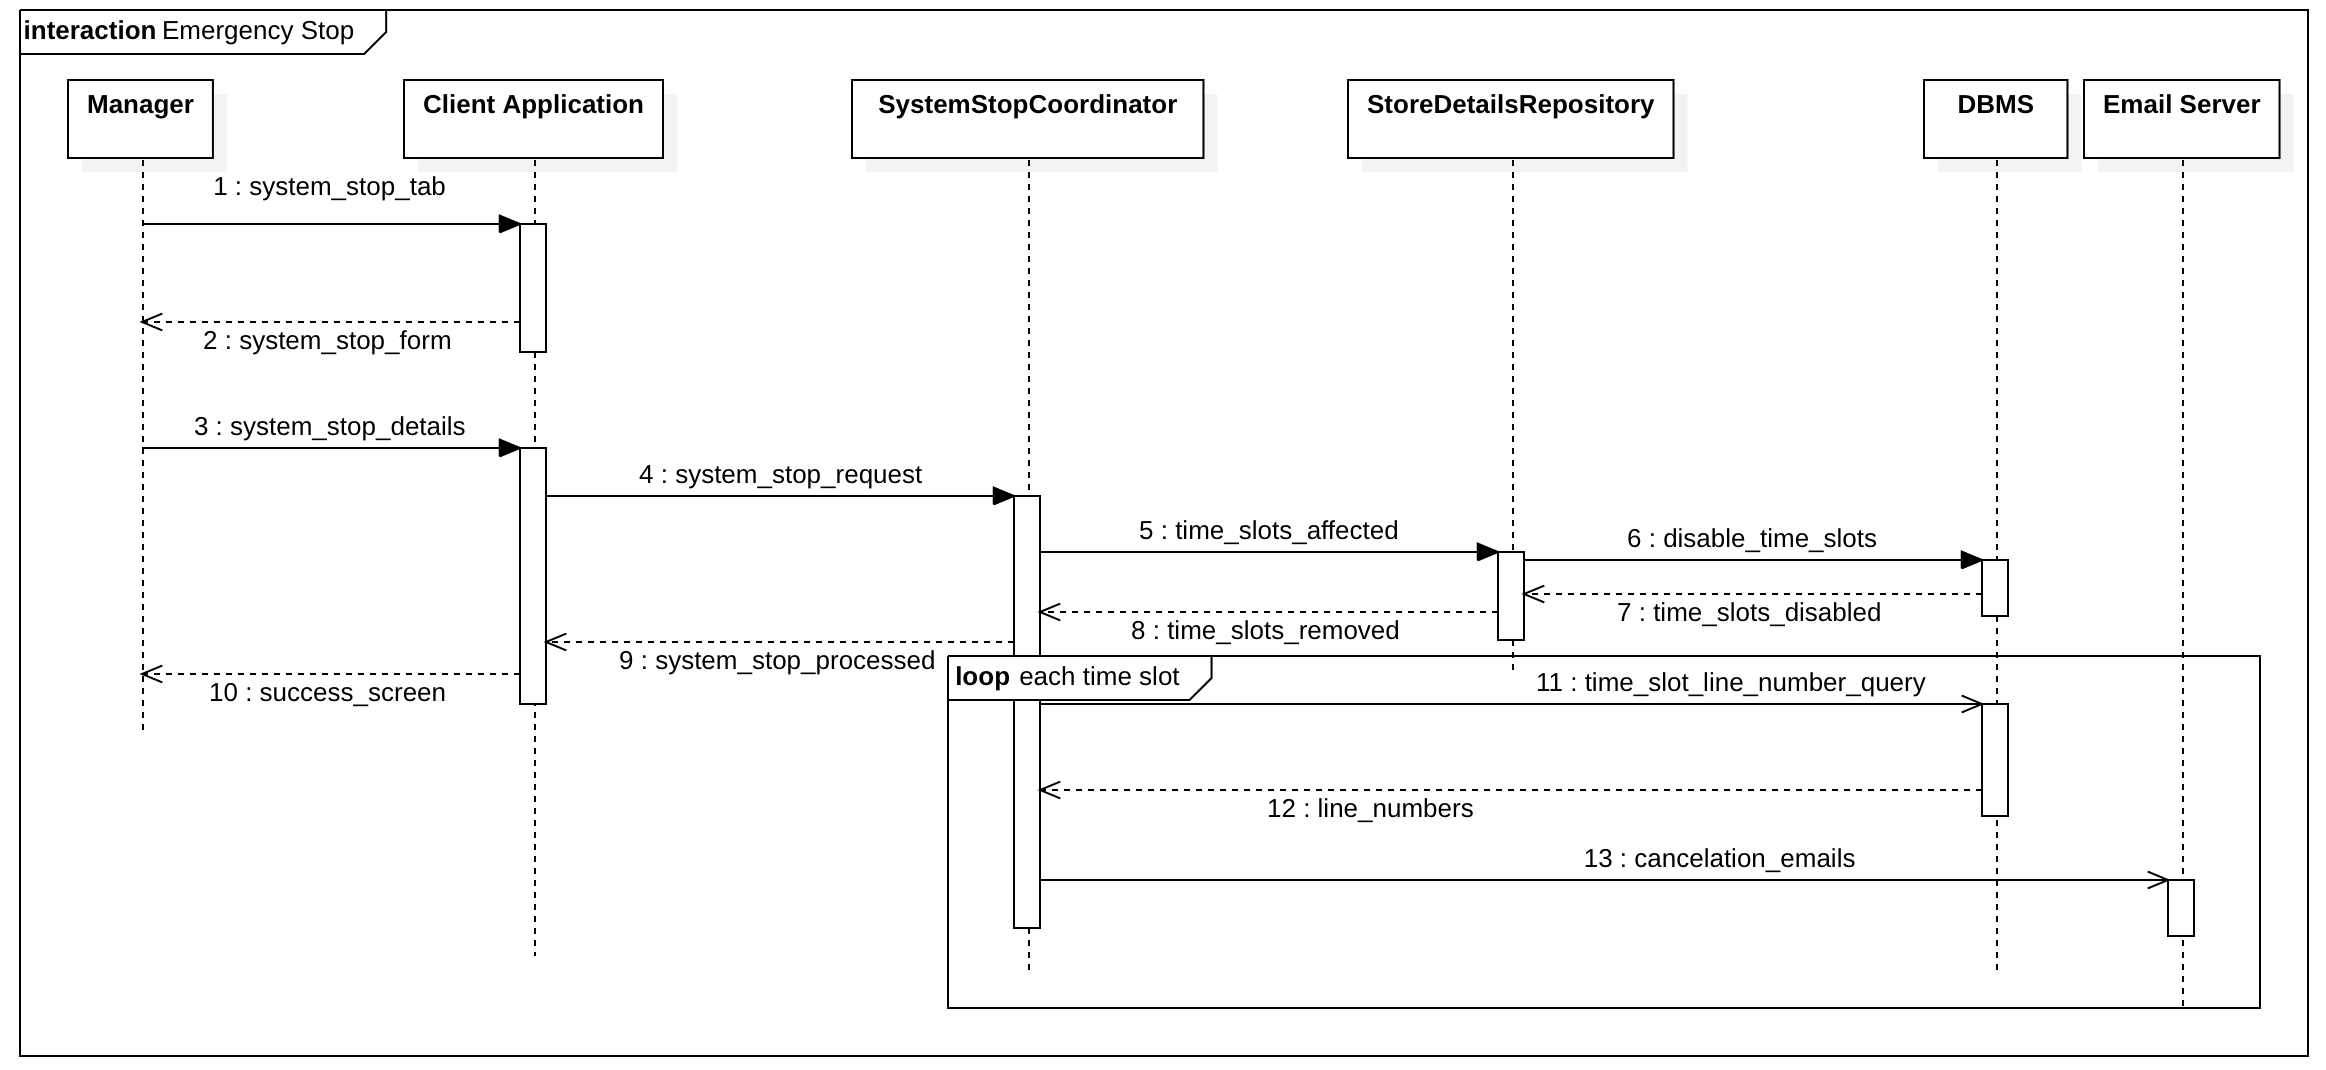
\includegraphics[height=0.4\textwidth]{Images/SequenceDiagrams/EmergencyStop.png}
    \caption{Sequence Diagram for Emergency Stop}
    \label{fig:SDEmergencyStop}
\end{figure}
\nameref{fig:SDEmergencyStop} demonstrates the flow of communication between different components of the system to create a emergency system stop, that can be issued immediately or scheduled to a future day, by the manager.
When the manager wants to open the "System Stop" tab, the application renders a form providing input fields for details regarding the system stop, which is about whether it is immediate or when it shall be performed.
After the manager providing the details of the stop, the application performs a request to the SystemStopCoordinator, the component responsible for handling system stop actions, which includes all the details provided by the manager.
The coordinator first initiates the transaction for disabling all the time slots affected by the specific request from the store by sending message to StoreDetailsCoordinator, which in turn sends the disabling query for all the timeslots of the specific store to the DBMS.
The DBMS then returns a message with the list of disabled time slots, which then the StoreDetailsRepository propagates back to the SystemStopCoordinator.
It shall be noted that, due to various reasons, the actual disabled time slots might be less than the affected time slots, since it can be the case that some of the slots were already disabled before this transaction.
After the disabling of the time slots an action receipt is returned to the CLup application indicating completion of the process, which in turn renders a success screen to the manager.
Meanwhile, the SystemStopCoordinator also starts sending email notifications for each time slot that has been removed from the store.
For each slot, a query to the DBMS is sent to determine the users that have already booked like numbers for the specific slot.
When the response from DBMS is retrieved the SystemStopCoordinator starts sending emails to all those users, through the Email Server component.

\subsubsection{Update Store Information}
\begin{figure}[H]
    \centering
    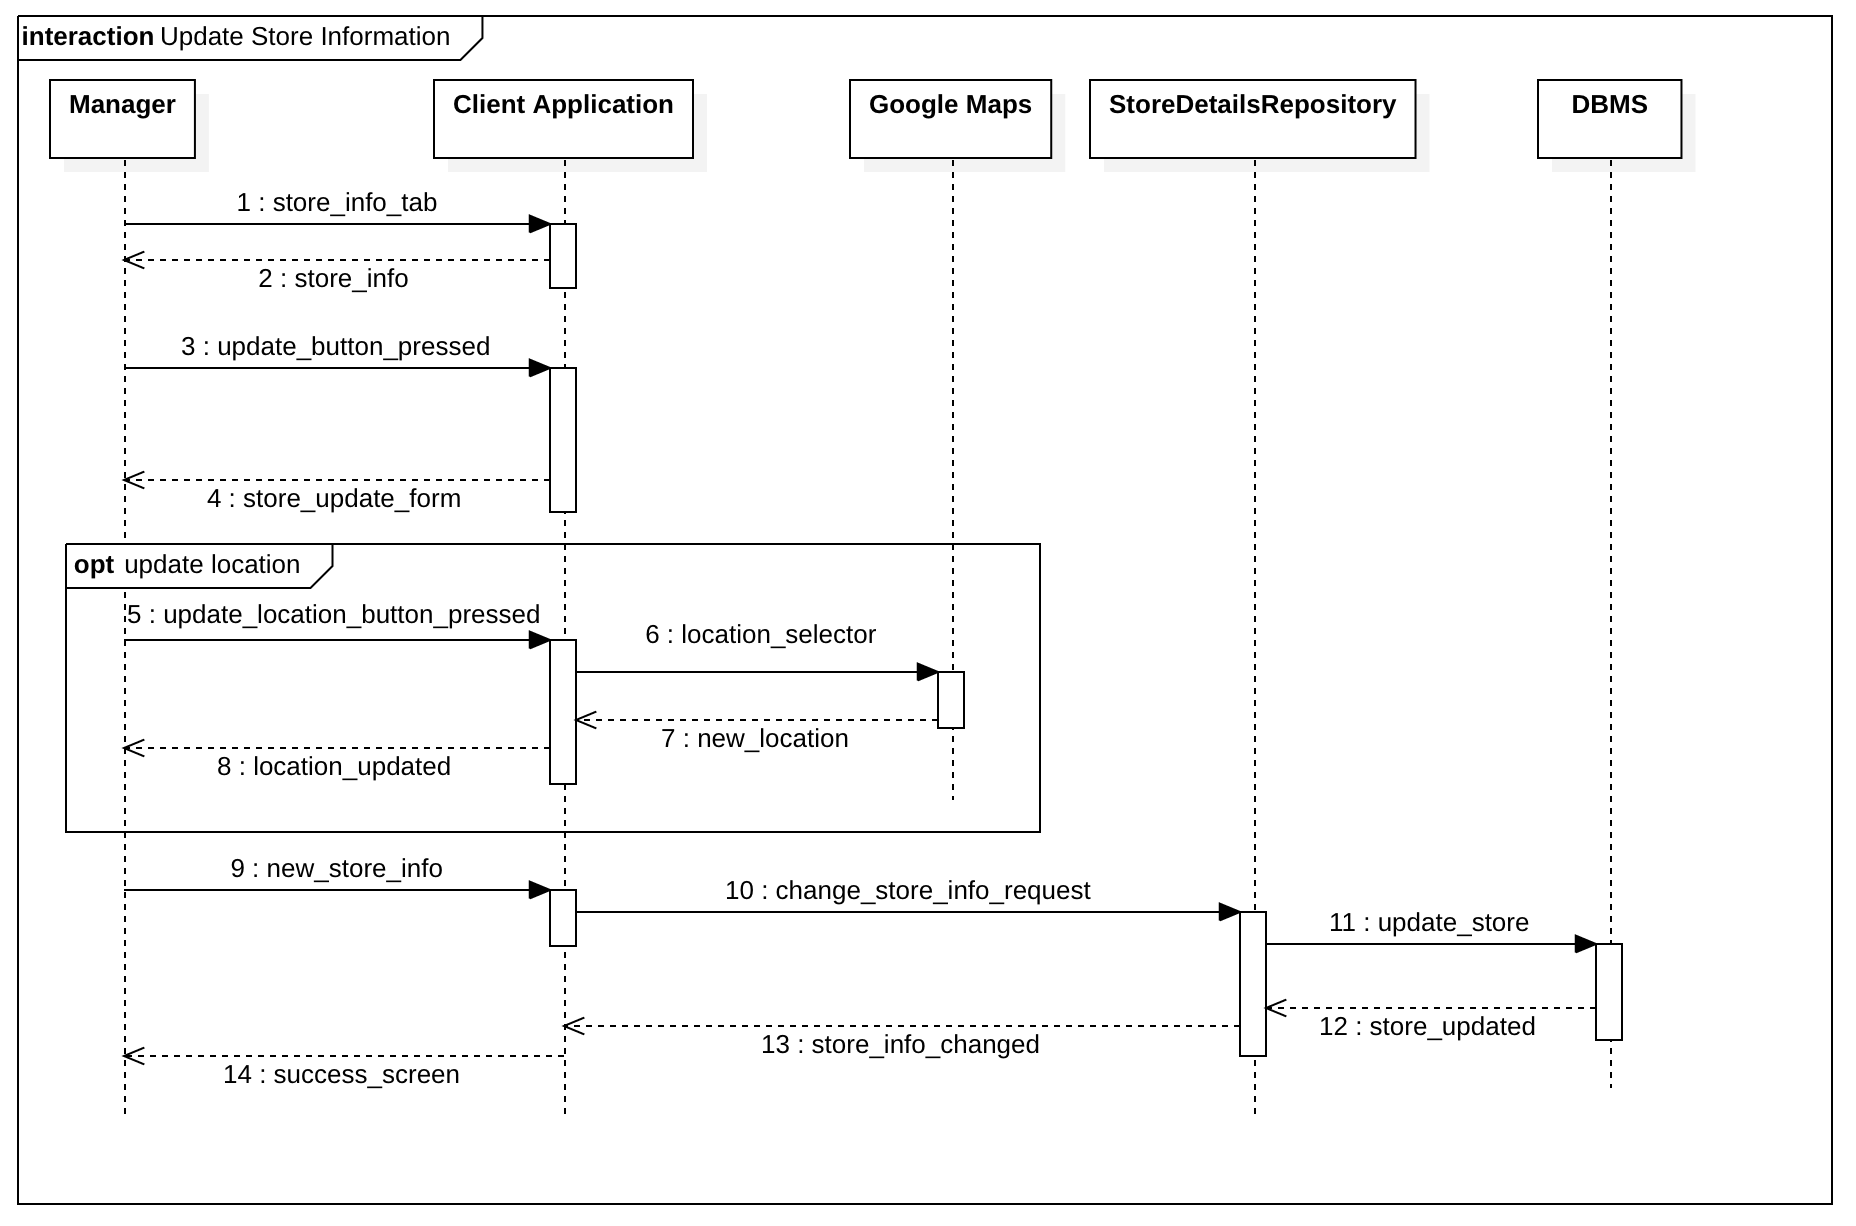
\includegraphics[height=0.4\textwidth]{Images/SequenceDiagrams/UpdateStoreInformation.png}
    \caption{Sequence Diagram for Update Store Information}
    \label{fig:SDUpdateStoreInformation}
\end{figure}
\nameref{fig:SDUpdateStoreInformation} shows the interactions between the components of the related parts of the system to update store information by the manager.
When the manager requests to see the information for the store, the client application displays the related information with an update button.
Upon trigger of the button, the CLup Application shows the editing form for the general information about the store, with the current values already pre-filled.
Optionally, from this moment, if the manager wants to update the store's location, they can do so by pressing the update location button, which in turn, triggers the Google Maps component to show the location selector.
Once the manager sets the new location, the service returns the new location selected by the manager, to be updated on the form.
After all the necessary changes are made, the manager submits the form which makes the CLup Application perform a request to the StoreDetailsRepository.
The StoreDetailsRepository, after processing the data, calls the DBMS to update the database entry for the store.
Once the updated message is retrieved from the DBMS, the message propagates through the calls and a success screen is shown to the manager.
\subsubsection{Monitor Customers}
\begin{figure}[H]
    \centering
    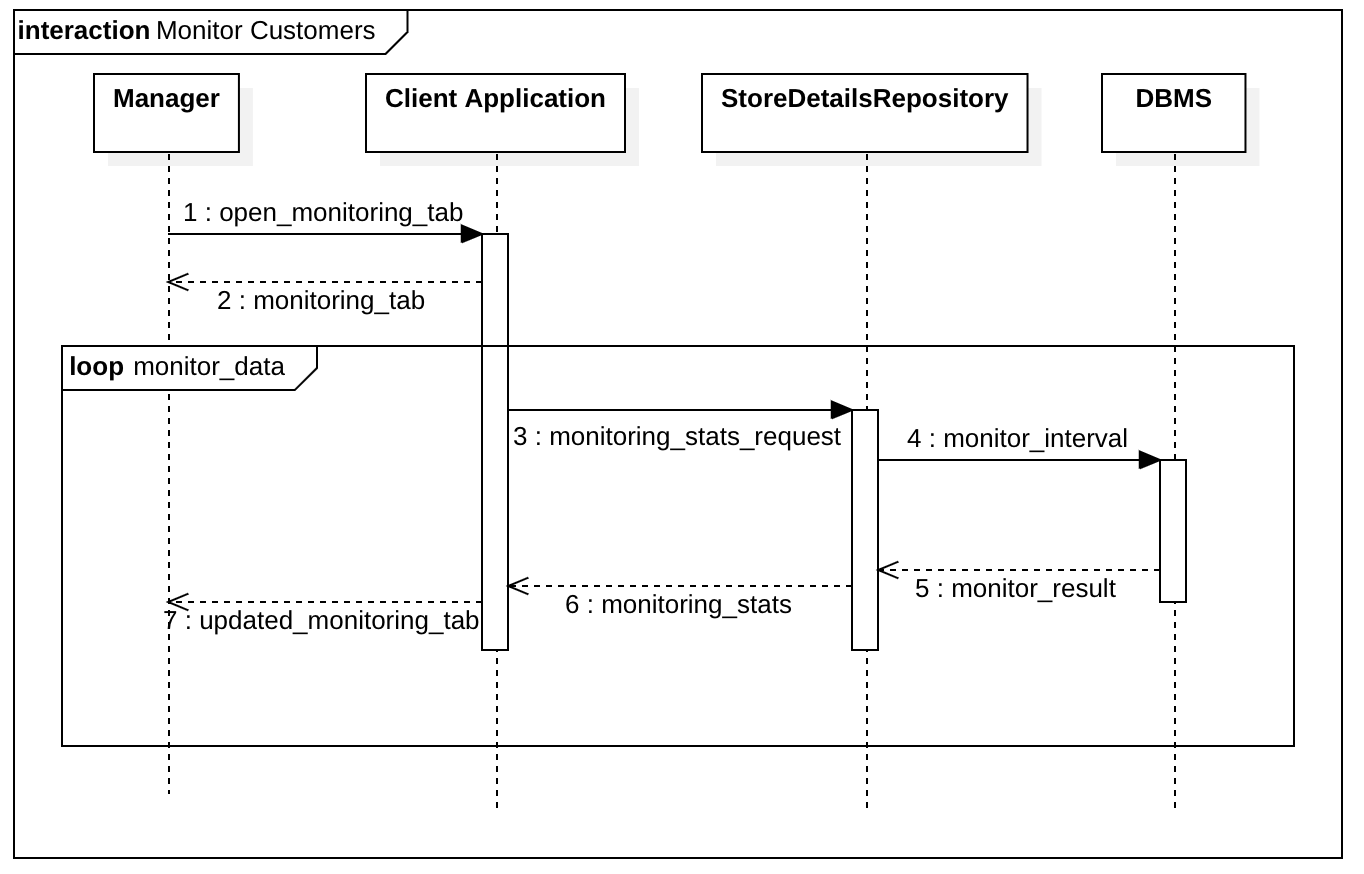
\includegraphics[height=0.4\textwidth]{Images/SequenceDiagrams/MonitorState.png}
    \caption{Sequence Diagram for Monitor State}
    \label{fig:SDMonitorState}
\end{figure}
\nameref{fig:SDMonitorState} displays the interactions between the components of the system required to enable general monitoring of the amount of customers in the store by the manager.
When the manager wants to see the monitoring results for the store, the client application shows the store monitoring tab to the manager.
Meanwhile, the client application requests the related monitoring statistics from the server continuously, for which the request is handled by the StoreDetailsRepository.
The repository queries the database through the monitor interval function, passing the interval requested by the client application.
The database then returns the view for the monitoring result given the specific time interval, which in turn is passed to the client app.
As the client app retrieves the data, it updates the monitoring tab that the manager sees with new information, and continues with the loop.

% Clerk
\subsubsection{Grant Access} %TODO: Hrvoje
\subsubsection{Generate Guest Ticket} % TODO: Hrvoje

% You can use sequence diagrams to describe the way components interact to accomplish specific tasks typically related to your use cases

% Main use cases with sequence diagrams indicating relations of each diagram to one another.

\subsection{Component interfaces}
% TODO: Ozan for 2 week
In the following UML Class Diagram, the main interactions between components have been shown.
The diagram's scope is mainly the application server and the peripheral services that the server communicates to function correctly.
The front-end interfaces are not included as they only act as a mean of communicating the server functions to the end user, thus they do not include any specific functionality implemented.
This diagram presents many details regarding the interactions between the system components, however this diagram does not provide a skeleton for the actual implementation, since its sole purpose is to demonstrate the significant integrations between components.
Thus, it shall only be seen as a guide to implement the actual system.
In this diagram, all user facing interfaces' (LineNumberManager, StoreManager and UserManager) functions are assumed to retrieve the user calling as an implicit argument, thus authorization aspect is not reflected in this diagram for simplification.
In this diagram, many entities in function inputs are represented as they are (like Store, User, TimeSlot, etc \ldots), however for optimization purposes the actual implementation may use the specific IDs of each entity instead of passing the whole object.
The DateTime used in this diagram is a general name for any implementation for a structure to store a specific time conforming to the standard \cite{}.
In the diagram, representations for errors that might be returned from the operations are omitted (such as access right problems, network errors), for simplification purposes, along with specific errors (such as conflicts).
% Diagram here

Details regarding the interfaces in () are:
\begin{itemize}
    \item \textbf{JPA}: \\
    This component represents the functionalities that are implemented in the JPA code that is used to communicate with the database.
    It should be noted that these operations represent the first abstraction layer of the underlying database towards the data model, thus they consist of the most primitive building blocks to realize the actions to be performed on the domain.
    The underlying realization of the SQL queries while executing these operations are also considered, and one-to-one mapping between the operations and queries are implemented in order to compensate for the atomicity of the calls made to this interface.
    The \textit{getDetails} methods are implemented to provide an interface to resolve the lazy entities of \textit{LineNumber}s and \textit{Store}s, such as \textit{productCategories} or \textit{partnerStores}.

    \item \textbf{EmailDispatcher}: \\
    This component represents the interface with the E-mail Client to send emails through SMTP.
    Since it has only one functionality regarding the scope of our system (sending emails to customers), the sole function of it is represented in this diagram.
    \item \textbf{OccupancyForecaster}: \\
    This component updates the OccupancyForecasts of each store whenever is necessary.
    In order to decrease the overhead of constantly updating the forecasts, this component is to work asynchronously when the transactions on the system are minimal.
    The only operation exposed by this interface allows the stores to be registered for updates.
    \item \textbf{UserManager}: \\
    This component is responsible for handling all transactions regarding the system's users, including authentication.
    The object LoginCredentials is implemented in order to provide an abstraction over the authentication method to allow flexibility to swap the method for different markets and times.
    The method \textit{login} returns an AuthenticationToken, which is also unspecified to allow flexibility for different methods, such as Bearer tokens or JWTs.
    While the customers are created using the \textit{register} operation, managers and clerks of the system are created using the \textit{createStaffMember} operation, while the first manager of a store is created along with the store, in the \textit{initializeStore} function of the StoreManager.
    None of the users can delete themselves, only managers can delete staff from the store that they manage, and all the staff users are linked to a specific store.
    These decisions are made to ensure that all stores have at least one manager at all times, including their creation, and simplified management of roles (as all users will have at most one role in the system).
    \item \textbf{LineNumberManager}: \\
    This component is responsible for handling all the transactions made with the line numbers on the system.
    The operations for creating line numbers (\textit{generateLineNumber}, \textit{getInmediateLineNumber} and \textit{bookLineNumber}) may not be able to generate line numbers, due to system being stopped, maximum capacity is reached or set reservation limits are reached.
    The operation \textit{check} is called by the Clerks to allow customers in and out of the system, having its first argument indicate the direction.
    The actual realization of this argument could be a boolean value, an enum or a custom typing instead of a string with two values.
    \item \textbf{StoreManager}: \\
    This component is responsible for handling any update or query regarding a store, including creation, forecasting and monitoring.
    The \textit{updateStore} operation is modeled as it retrieves all the changes to the store, however the operation can also be receiving partial updates of the store data instead of the whole store data, so that the network load for the request can be reduced.
    The operations to update the related data (\textit{updateTimeSlots} and \textit{updatePartnerStores}) feature \textit{operation} arguments of type CUDOperation (CUD stands for Create, Update, Delete), which indicate that the request may not only be about updating a field or a specific instance of the given entity, but also to create new ones and remove existing ones.
    Some operations may cause an invalidation of customer's tickets, leading to a potential loss of customers.
    In order to prevent this from happening, the operations that might lead to this (\textit{updateTimeSlots} and \textit{systemStop}) feature a \textit{force} argument.
    The call would produce an error if the force argument is not given, and there are customers who have booked any line numbers in an affected time slot.
    The operation \textit{monitor} features an optional argument of 2 \textit{DateTime}s.
    If these are not provided, the operation is to return the live monitoring result (the flow of customers in realtime).
\end{itemize}
% Class diagram with only methods demonstrating how components interact with each other.
% Also an ER or Class diagram to indicate data.

The UML Class Diagram below describes the model of the system.
In order to be consistent with the diagram in the RASD, and to demonstrate views and enumerations, the Class Diagram was preffered over an Entity-Relationship Diagram.
For the sake of simplicity, the unique \textit{id}s of entities are not shown.
These \textit{id}s don't have any special requirements, thus can be auto-generated using built-in generation mechanisms existing in SQL database implementations.
The diagram is similar to the one in RASD, however features more implementation details.

% Diagram here

The \textbf{LineNumberStatus} indicates the current \textbf{LineNumber}'s status.
When the line number is generated, it should be initialized with the status \textit{AWAITING} which indicates that the customer didn't yet enter the store.
After the entrance of the customer, the line number enters to the state \textit{VISITING} to indicate that the customer has successfully arrived at the store and currently shopping.
When the customer leaves, the ticket becomes \textit{VISITED} to indicate a successful exit from the store.
If, for any case, the customers' ticket becomes invalid (due to time slot changes, system stop or ticket timeout), the ticket is marked as \textit{EXPIRED}.
The \textit{entryTime} and \textit{exitTime} are used to store the time interval that the customer has entered to the store and exited, to allow better monitoring.
The features to time out the tickets after some time, reservation limiting, and product category selection to increase granularity of visit can be enabled or disabled by the manager.
Thus, on the class \textbf{Store} attributes related to these features (\textit{reservationLimit}, \textit{timeoutMinutes} and \textit{productCategories}) have to multiplicity of $0..1$ to demonstrate this ability.
The representation of the location on the diagram is given as the Latitude and Longitude on the Earth, according to ISO 6709.
% TODO: Reference
The latitude and longitude are limited with 4 decimal points, since this provides a precision of at least 12 meters on the Earth, which is in the range provided by $D_{5}$.
% Source: https://en.wikipedia.org/wiki/Decimal_degrees
The \textbf{OccupancyForecast} is implemented as an estimated indication of amount of customers per time slot.
Since the main purpose of this component is to provide an idea to the customers about how crowded the store is in a certain time slot, the granular implementation is the part of the \textit{MonitorResult} view instead.
The \textit{MonitorResult} view provides the amount of customers that has visited the store from and to a specific time, which may or may not correspond to a \textbf{TimeSlot}.
This view is used to implement a basic monitoring view for the \textbf{Manager}.
The \textbf{ProductCategory} class features an \textit{locatedAt} property in order to help customers know where to find a specific category.
The \textbf{InStoreLocation} class provides a name for the location in the shop and a description of how to reach there.
It may also feature an image of a sketch, diagram or a map indicating the location, considering many large chains already has such a facility.
Some store may feature these in an interactive format in their websites or in any other format, however considering that the category location is static, such dynamism is not required.
In order to facilitate, a screenshot may be provided in the system of such interactive representation.

\subsection{Selected architectural styles and patterns} % Do as we proceed

\subsubsection{Thick-Server}
Many transaction that occur on the system requires checks to be performed on data, thus these transactions needs to be handled on the server.
Although basic data validation (such as verifying e-mail addresses conform to RFC 822) is possible and better yielded to the client, consistency checks (such as preventing customer overflow) requires a thick-server model.
% TODO Reference: RFC822: https://tools.ietf.org/html/rfc822
% All transactions occur in server side
\subsubsection{Logical Sharding}
Since the data on the system is either strictly location dependant (stores and any subsidiaries exist in a specific province or country) or changes location rarely (Customers don't switch countries or provinces often), the data plane can be logically sharded based on location if necessary.
With logical sharding, the system can scale without hitting any bottleneck regarding database application limits.
Furthermore, the data tier can be provisioned on locations closer to the sharded target location, thus reducing the network latency.

% Due to the definite split based on location for our data, we can implement logical sharding to split our databases based on zones, which will decrease the latency to retrieve information
\subsubsection{Lazy Loading}
Store, the largest entity contains foreign fields that needs multiple accesses to fully retrieve, which would decrease the overall performance of the system, as PartnerStore, TimeSlot, Categories .
Thus, this problem necesitates the implementation of lazy loading for such entities on the ORM level.

\subsubsection{Service-Oriented Architecture}

% Our server architecture's components are split into different services, accessible to outside world and each other through procedure calls and HTTP requests.

Many services and options that our system provides can be split into different services, sharing the same database.
However, since there is no scalability concern, due to the ability to perform logical sharding, or version compatibility problems, since all system components are planned to exist on same machine, there is no need to implement microservices.
Thus, the system is implemented with Service-Oriented Architecture, which allows the developers to split the implementation of functionalities belonging to different domains, while not requiring to implement containerization or provisioning of multiple databases and data brokers.
The services are exposed to each other through dependency injection and exposed to outside world via HTTP.

% Please explain which styles/patterns you used, why, and how
\subsection{Other design decisions} % Do as we proceed.
\subsubsection{ORM}

To facilitate the development of the system, instead of hand crafting database queries, an ORM shall be used to further improve development speed and security, as many ORM implementations support the prevention of SQL related attacks.

\subsubsection{ACID}

The database operation is based on the ACID principles, since the core system doesn't require asynchronous data synchronization with any other external components.
Furthermore, as the system will implement Logical Sharding, there wouldn't be a need for increasing the partitions of the database, thus the system will not suffer from the limits of the CAP theorem.
% \subsubsection{Single Sign-On}

% In order to decrease the security risks and decrease the cost, the system is to implement SSO

